
\section{\acl{dl}-Based \ac{ser}}

This section presents the exploration of using deep learning classifiers for audio-based emotion recognition, focusing on the use of various features for the classification task.

\subsection{\acl{dl} Features}

Initially, three different features were extracted from the raw audio signals, using the Librosa library. The numeric values of the extracted features were saved into a Pickle file, while the visual representation of the feature was saved as a Portable Network Graphic (PNG) file. The PNG file was generated using a Matplotlib figure with 100 dots per inch, without the axis and the frame. The color map used was \textit{viridis\_r}.

The 2D deep learning models employed in this study required the input data to possess consistent dimensions. To this end, the numeric data of every feature used only the first 6 seconds of every audio file, with shorter audio signals padded with trailing zeros to achieve the required length. For the 3D models that performed classification based on the PNG images, the full signal is utilized.

The first feature explored was the spectrogram. The Short-time Fourier transform was used to calculate the spectrogram, using a windowed signal length of 2048, after padding with zeros. This resulted in matrices with a dimension of $1025x188$. The amplitude spectrogram was converted to a dB-scaled spectrogram, which was then used for the PNG file.

Another feature explored was the Mel Spectrogram. For this, the previously calculated spectrogram was mapped onto the mel scale, using 256 Mel bands. This resulted in matrices with a dimension of $256x188$. The dB-scaled Mel Spectrogram was also used for the PNG file.

The third feature explored was the \ac{mfccs} as they are commonly used for audio signal processing tasks due to their ability to capture the spectral characteristics of audio signals. 40 \ac{mfccs} were extracted from the previously calculated Mel Spectrogram, resulting in matrices with a dimension of $40x188$.

These three used features are displayed in figure \ref{fig:dl_features}.

\begin{figure}[H]
	\centering
	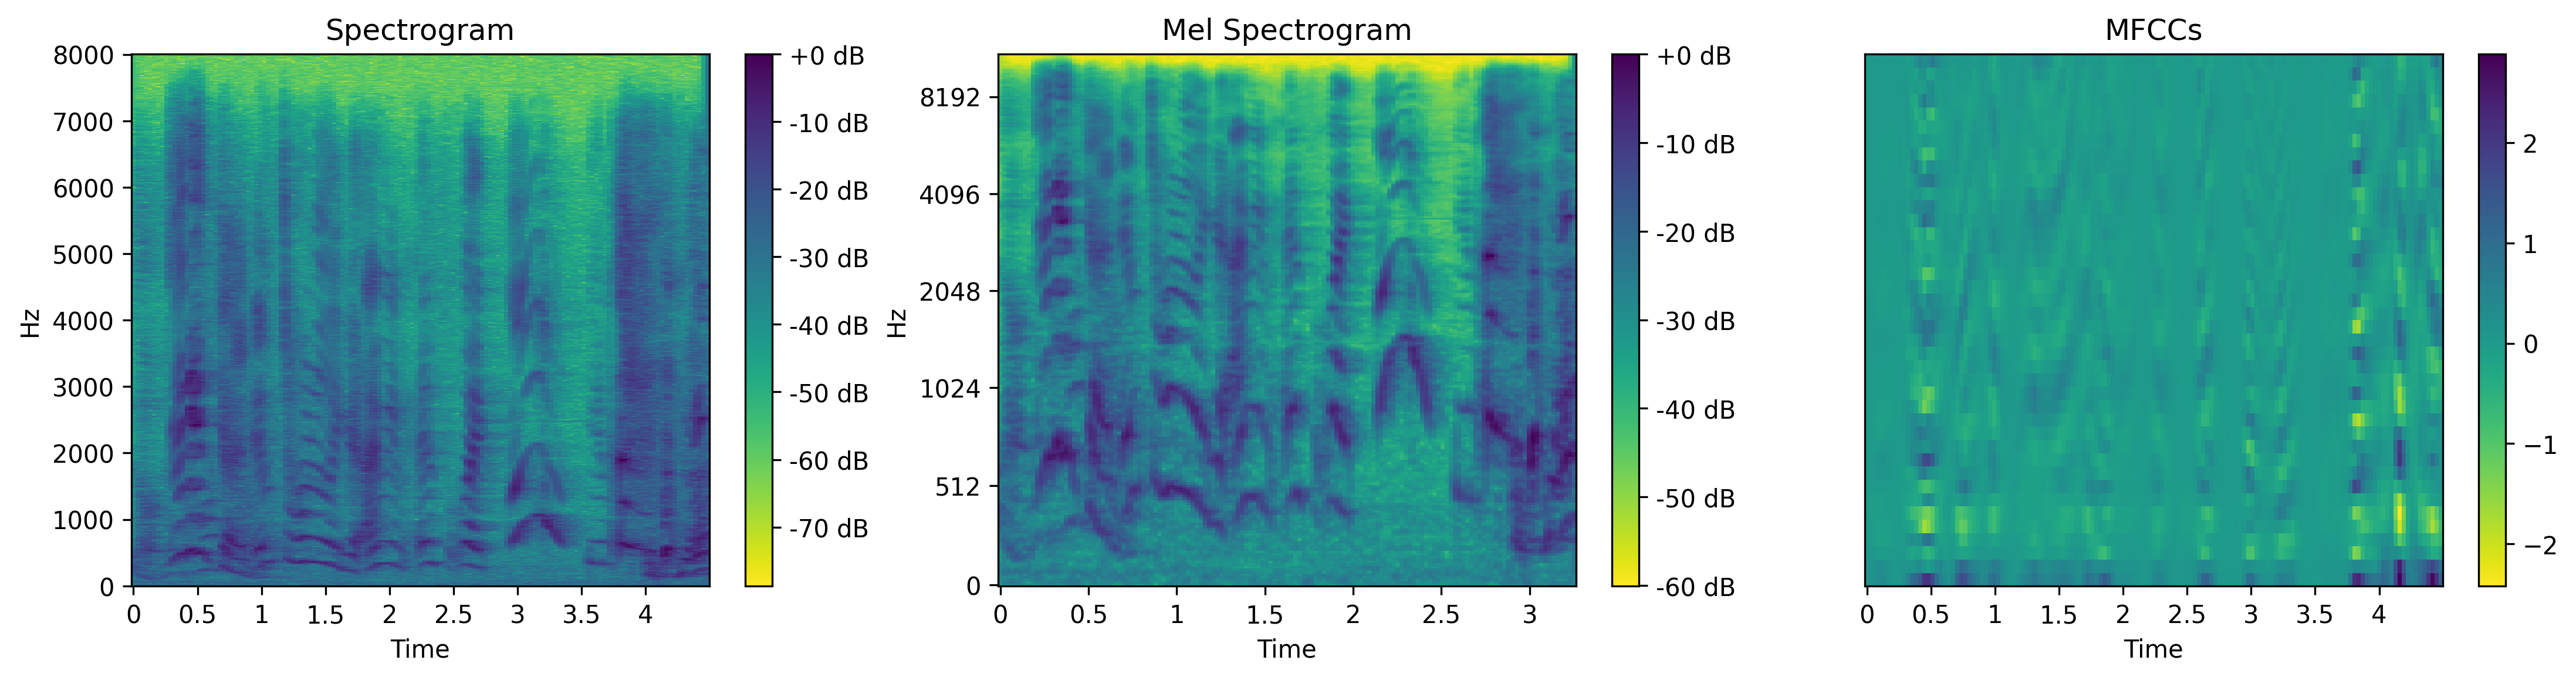
\includegraphics[width=\textwidth]{figs/4_4_deep_learning/features.png}
	\caption{Graphical representations of the features used as input for the \ac{dl} classifiers.}
	\label{fig:dl_features}
\end{figure}



\subsection{Classifiers Evaluation and Selection}

\subsubsection{Evaluation Strategy}

To evaluate the performance of the classifiers, 5-fold \ac{cv} was performed using the stratified K-fold strategy to preserve the percentage of samples for each class, following the same strategy for the traditional approach. The models were trained for 80 epochs, with a batch size of 128 and a learning rate decay of 10\% every 10 epochs. The Adam optimizer was used for all models with a learning rate of 0.001.

The evaluation of the classifiers was done based on various metrics including accuracy, precision, recall, and macro F1-score. The training time was also annotated and the corresponding confusion matrices were also plotted, present in the appendix \ref{TODO}. These metrics were computed using the unweighted average across the 5 folds, to give an overall performance overview of the classifier.

\subsubsection{Classification of Numeric Data}

In order to classify the numeric data, we employed two deep learning models that take as input the 2D matrices with the corresponding dimensions of the features previously described.

The first model is a deep \ac{cnn} based on the architecture proposed by \citeauthor{Mustaqeem2019} \cite{Mustaqeem2019}. It comprises 7 convolutional layers followed by 2 fully connected layers to perform the classification task. To prevent overfitting, the model includes regularization techniques such as batch normalization after each convolutional layer and a total of three dropout layers. The authors used spectrograms as input for the model and achieved an unweighted average accuracy of 72\% by performing 5-fold \ac{cv} on the \ac{iemo} dataset.

The second model is a combination of a \ac{cnn} and a \ac{rnn} in a single architecture, based on the work of \citeauthor{ma18b_interspeech} \cite{ma18b_interspeech} published in \citeyear{ma18b_interspeech}. This model consists of 2 convolutional layers, each followed by batch normalization. The output from these layers is then given to a bidirectional \ac{lstm} layer followed by a dropout layer and finally, a dense layer with 4 units to classify the emotions. The authors used log spectrograms as input for the model and achieved an unweighted average accuracy of 64.22\% by performing 5-fold \ac{cv} on the \ac{iemo} dataset.

Both models utilize an Adam optimizer with a learning rate of 0.001, a sparse categorical cross-entropy loss, and accuracy as the evaluation metric.

\subsubsection{Image Classification}

In our study of deep learning-based \ac{ser} using images, we utilized transfer learning techniques with three different pre-trained models: ResNet50, VGG16, and Xception.

ResNet50, VGG16, and Xception are popular deep \ac{cnn} that have shown outstanding performance in various computer vision tasks, including image classification. We used the pre-trained versions of them on the large-scale ImageNet dataset, which contains millions of labeled images belonging to thousands of different classes. This means their weights and biases have already been adjusted for the ImageNet dataset, and they have learned how to extract meaningful features from images, which helps improve the accuracy and generalization ability of the models, as it allows them to recognize patterns and shapes that are common across a wide range of images.

To prepare the data for these models, we loaded the images with a dimension of $224x224x3$ using the TensorFlow Keras \textit{load\_img} function from the \textit{preprocessing.image} module. The images were then converted into arrays using the \textit{img\_to\_array} function from the same module. In addition, before inputting the data into the models, we applied the respective preprocessing technique for each classifier. For example, we used the \textit{preprocess\_input} function from the Tensorflow  Keras \textit{applications.resnet50} module for the ResNet50 classifier.

To apply the transfer learning technique, all layers of the chosen model were frozen, and a new Dense layer with 64 units with \textit{relu} activation was added to the model. A Dropout layer with a 0.5 rate was then included to avoid overfitting, followed by a Dense layer with 4 units with \textit{softmax} activation to output the predicted emotion.

Through the implementation of these pre-trained models with transfer learning, we aim to harness their robust feature extraction abilities and significantly reduce the training duration required for the inherently computationally intensive 3D classification task at hand.


\subsubsection{Results and Conclusions}

The experiments were conducted using transfer learning with pre-trained models on a Tesla P4 GPU through the Google Colab service. Table \ref{tab:dl_models} summarizes the results of the experiments conducted with all classifiers evaluated.

Among the classifiers evaluated, the ResNet50 model stood out as the most effective, ranking in the top 3 in most metrics except prediction time, as it is a heavier model compared to Xception and VGG16 models.

In terms of the input feature used, while the spectrogram image feature attained the highest average accuracy with the Resnet50 model, the mel spectrogram feature achieved the best overall performance across the other evaluated models. Furthermore, the image of the mel spectrogram obtained the second-highest accuracy with the Resnet50 model and displayed a smaller standard deviation, indicating that it performed comparably well in all \ac{cv} folds.

Despite this, we decided to utilize the spectrogram image as our input feature. This decision was based on the fact that the mel spectrogram is a variation of the spectrogram that uses a mel-scale to convert frequency units to a logarithmic scale that better approximates human auditory perception. This conversion can result in the loss of some information that is only present in the original spectrogram, particularly in the higher frequencies. Therefore, we reasoned that by using the spectrogram image as our input feature, we may be able to preserve some important information that is lost in the mel spectrogram.

Therefore, based on the results obtained, we conclude that the Resnet50 model with spectrogram images as input is the best candidate for the \ac{dl} model for the \ac{ser} task. It is also essential to acknowledge that \ac{dl} can yield even better results with more extensive models' hyperparameter tuning, which would demand more computation time and power for their development and evaluation.

\begin{table}[H]
	\centering
	\caption{\ac{dl} classification models performance on \ac{iemo}.}
	\label{tab:dl_models}
	\resizebox{\textwidth}{!}{%
		\begin{tabular}{llrrrrrr}
			\toprule
			Feature & Model & Accuracy & Macro F1 & Precision & Recall & \ac{mcc} & Prediction Time\\
			\midrule
			
			Spectrogram Image & Resnet50 & 58.24$\pm$2.20 & 58.97 & 59.38 & 59.00 & 0.436 & 20.78 \\
			
			Mel Spectrogram Image & Resnet50 & 57.95$\pm$1.36 & 58.71 & 59.27 & 58.49 & 0.430 & 20.92 \\
			
			MFCCs Image & Resnet50 & 56.59$\pm$0.45 & 57.29 & 58.59 & 56.67 & 0.410 & 23.19 \\
			
			Mel Spectrogram Image & VGG16 & 55.07$\pm$2.23 & 55.82 & 56.77 & 55.29 & 0.389 & 12.04 \\
			
			MFCCs Image & VGG16 & 54.73$\pm$1.47 & 55.51 & 56.32 & 55.14 & 0.386 & 10.89 \\
			
			Spectrogram Image & VGG16 & 54.28$\pm$0.90 & 55.21 & 55.85 & 54.87 & 0.379 & 12.16 \\
			
			Mel Spectrogram Image & Xception & 53.10$\pm$1.42 & 53.84 & 54.27 & 53.68 & 0.364 & 19.06 \\
			
			MFCCs Image & Xception & 52.78$\pm$0.96 & 53.47 & 54.10 & 53.22 & 0.359 & 18.33 \\
			
			Spectrogram Image & Xception & 52.78$\pm$1.54 & 53.51 & 53.48 & 53.62 & 0.361 & 19.55 \\
			
			Spectrogram &  2D-\ac{cnn} & 50.12$\pm$0.91 & 50.04 & 52.98 & 49.65 & 0.320 & 21.2 \\
			
			Mel Spectrogram & 2D-CNN \& \ac{rnn} & 48.02$\pm$1.14 & 47.93 & 48.60 & 48.47 & 0.298 & 20.05 \\
			
			MFCCs &  2D-\ac{cnn} & 46.70$\pm$0.85 & 47.13 & 49.53 & 46.75 & 0.275 & 5.18 \\
			
			Spectrogram & 2D-CNN \& \ac{rnn} & 46.01$\pm$1.77 & 47.09 & 47.37 & 46.87 & 0.269 & 32.07 \\
			
			MFCCs & 2D-CNN \& \ac{rnn} & 45.56$\pm$1.15 & 46.26 & 46.29 & 46.25 & 0.263 & 12.29 \\
			
			Mel Spectrogram &  2D-\ac{cnn} & 32.51$\pm$1.13 & 21.34 & 20.38 & 30.26 & 0.102 & 9.21 \\
			
			\bottomrule
		\end{tabular}%
	}
\end{table}

\paragraph{Chosen Model: ResNet50}

ResNet50 is a deep neural network model used for image classification tasks. It is based on a residual network architecture that allows for the training of very deep neural networks. The model consists of 50 convolutional layers and uses skip connections to facilitate the flow of information directly from one layer to another, enabling the network to learn more complex representations of the input data. This helps to overcome the problem of vanishing gradients and enables the network to be trained deeper.

ResNet50 has achieved \ac{sota} performance on a range of image classification tasks, such as object recognition and image segmentation. It is a popular choice for transfer learning, where pre-trained models can be fine-tuned for specific tasks with smaller datasets.

Despite its high accuracy, the ResNet50 model has a large number of parameters and requires significant computational resources to train. However, pre-trained models on different datasets are widely available in \ac{dl} frameworks like TensorFlow and PyTorch. These pre-trained models can be used as starting points for specific image classification tasks and fine-tuned with smaller datasets, reducing the time and computational resources required for training.

\paragraph{ResNet50 Implementation}

The code snippet \ref{dl:code} implements in Python our transfer learning approach using a ResNet50 model, pre-trained on the ImageNet dataset with a total of 23,719,108 parameters. However, in this implementation, only 131,396 parameters are trainable, which corresponds to the new layers added.

First, the ResNet50 model is loaded using the Keras API from TensorFlow, with the "\textit{weights}" parameter set to "\textit{imagenet}" to load the pre-trained weights, "\textit{include\_top}" set to False to remove the last classification layer, and "\textit{pooling}" set to "\textit{avg}" to obtain a global average pooling layer as the output. The pre-trained model is then set to be non-trainable.

As mentioned previously, the input layer is defined with the spectrogram image shape, and the output of the pre-trained model is fed into a new dense layer with 64 units and ReLU activation. A dropout layer with a rate of 0.5 is added to reduce overfitting. Finally, the output layer consists of a dense layer with 4 units and softmax activation, corresponding to the 4 possible emotions to be recognized. The model is then compiled with the Adam optimizer, sparse categorical cross-entropy loss, and accuracy as the evaluation metric.

With this implementation, we can take advantage of the pre-trained model on a large dataset and fine-tune it for our specific \ac{ser} task.

\begin{listing}[H]
	\begin{minted}{python}
import tensorflow.keras as K
model = K.applications.resnet.ResNet50(weights='imagenet',
		input_shape=(224, 224, 3), include_top=False, pooling='avg')
model.trainable = False
inputs = K.Input(shape=(224, 224, 3))
x = model(inputs, training=False)
x = K.layers.Dense(64, activation='relu')(x)
x = K.layers.Dropout(0.5)(x)
outputs = K.layers.Dense(4, activation='softmax')(x)
model = K.Model(inputs, outputs)
model.compile(optimizer=K.optimizers.Adam(learning_rate=1e-3),
			  loss=K.losses.SparseCategoricalCrossentropy(),
			  metrics=['accuracy'])
	\end{minted}
	\caption{Python code for the selected ResNet50 classifier using the \ac{dl}-based \ac{ser} approach.}
	\label{dl:code}
\end{listing}


\paragraph{ResNet50 Advantages}

The ResNet50 model pre-trained on the ImageNet dataset has several advantages that make it a suitable choice for fine-tuning the task of \ac{ser} using audio spectrograms as input. One of the main advantages is its ability to handle the vanishing gradient problem that arises in deep neural networks with many layers, thanks to its residual connections. This makes it possible to train very deep neural networks without degradation in performance.

Additionally, the ResNet50 model's high accuracy in image classification tasks and relatively fast training time compared to other deep neural networks make it well-suited for large-scale tasks. Its architecture also facilitates implementing transfer learning, where the pre-trained model can be fine-tuned on new datasets with relatively little additional training data.

In conclusion, utilizing the ResNet50 model pre-trained on the ImageNet dataset and fine-tuning it for speech emotion recognition using audio spectrograms as input is an effective approach to achieve high accuracy in this task. The model's ability to handle the vanishing gradient problem, high accuracy in image classification, and fast training time make it a powerful and versatile tool for \ac{dl} applications.
